% !TEX program = pdflatex
\documentclass[aspectratio=169,10pt]{beamer}

% -------------------- Pacotes básicos --------------------
\usepackage[brazil]{babel}
\usepackage[T1]{fontenc}
\usepackage[utf8]{inputenc}
\usepackage{lmodern}
\usepackage{microtype}
\usepackage{amsmath,amssymb}
\usepackage{siunitx}
\usepackage{graphicx}

% -------------------- Estilo Beamer --------------------
\usetheme{Madrid}
\usecolortheme{default}
\setbeamertemplate{navigation symbols}{}
\setbeamertemplate{equation number}[default] % numeração de equações

% -------------------- Metadados --------------------
\title{Medidas e Algarismos Significativos}
\subtitle{Física Experimental}
\author{Prof. Rafael de Lima}
\institute{Departamento de Física --- CCT/UDESC}
\date{}

% -------------------- Atalhos --------------------
\newcommand{\abs}[1]{\left|#1\right|}
\newcommand{\Mean}[1]{\left\langle #1 \right\rangle}

\begin{document}

% -------------------- Capa --------------------
\begin{frame}
  \titlepage
\end{frame}

% -------------------- Roteiro --------------------
\begin{frame}{Roteiro}
\tableofcontents
\end{frame}

% =========================================================
\section{Motivação e ideias básicas}

\begin{frame}{Por que medir?}
\begin{itemize}
  \item A Física é uma ciência experimental: leis e modelos são confrontados com \textbf{medidas}.
  \item Medir bem envolve:
  \begin{itemize}
    \item escolher instrumentos adequados;
    \item registrar unidades e \textbf{incertezas};
    \item operar matematicamente sem “inventar” precisão.
  \end{itemize}
  \item Se toda medida tem erro, a prática do laboratório exige \textbf{tratamento cuidadoso} desses erros.
\end{itemize}
\end{frame}

\begin{frame}{Método científico (visão operacional)}
\begin{enumerate}
  \item Observação do fenômeno;
  \item Formulação de hipóteses;
  \item Teste por experimentos (medidas);
  \item Elaboração/ajuste de teoria.
\end{enumerate}
\end{frame}

\begin{frame}{Grandezas e unidades}
\begin{itemize}
  \item \textbf{Grandezas físicas}: quantidades mensuráveis (massa, comprimento, tempo, força, etc.).
  \item \textbf{Fundamentais} vs. \textbf{derivadas}.
  \item Sistema Internacional (SI) como referência.
\end{itemize}

\vspace{0.3cm}
Medir significa comparar com uma unidade padrão:
\begin{equation}
\label{eq:def_MG}
M(G)=\frac{G}{U},
\end{equation}
logo,
\begin{equation}
\label{eq:G_MU}
G = M(G)\,U.
\end{equation}
\end{frame}

\begin{frame}{Medida e “erro provável”}
Em qualquer medida, há incerteza. Um modo de expressar:
\begin{equation}
\label{eq:medida_com_erro}
G = \bigl(M(G)\pm \Delta M\bigr)\,U.
\end{equation}

\begin{itemize}
  \item A região de valores plausíveis fica entre
  \[
  \bigl(M(G)-\Delta M\bigr)U \quad \text{e} \quad \bigl(M(G)+\Delta M\bigr)U.
  \]
  \item O sinal \(\pm\) indica que a incerteza pode aumentar ou diminuir o valor.
\end{itemize}
\end{frame}

% =========================================================
\section{Algarismos significativos}

\begin{frame}{Medida direta e indireta}
\begin{block}{Medida direta}
Comparação \textit{direta} da grandeza com um instrumento (ex.: medir \(L\) com uma régua).
\end{block}

\begin{block}{Medida indireta}
Obtida por \textbf{operações} com medidas diretas (ex.: área \(A=L\times H\)).
\end{block}

\begin{equation}
\label{eq:area_exemplo}
A = L \, H.
\end{equation}
\end{frame}


\begin{frame}{7 Unidades Fundamentais}
   \begin{figure}
       \centering
       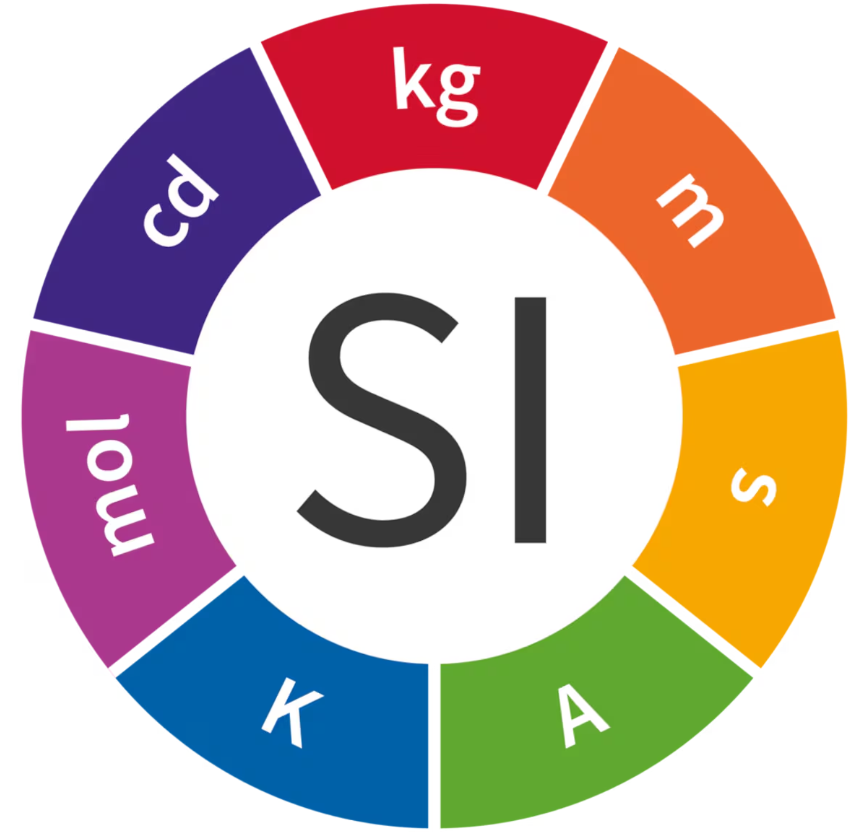
\includegraphics[width=0.5\linewidth]{7fundamentais.png}
   \end{figure} 
\end{frame}

\begin{frame}{O que são algarismos significativos?}
\begin{itemize}
  \item Ao ler um instrumento, você registra:
  \begin{itemize}
    \item todos os algarismos \textbf{certos};
    \item \textbf{mais um} algarismo \textbf{duvidoso} (estimado).
  \end{itemize}
  \item Esse último algarismo (duvidoso) \textbf{é significativo}.
  \item Qualquer algarismo \textbf{à direita} do duvidoso \textbf{não deve aparecer} no resultado.
\end{itemize}
\end{frame}




\begin{frame}{Leitura em réguas com escalas diferentes}
\begin{center}

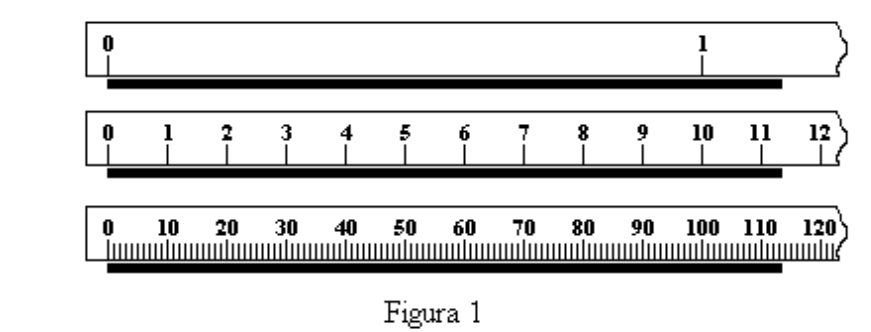
\includegraphics[width=0.85\linewidth]{reguas.png}

\fbox{\parbox{0.85\linewidth}{\centering
\textbf{[Figura 1: três réguas (dm, cm, mm) e a tira de papel]}\\
}}
\end{center}

\begin{itemize}
  \item Mais divisões na escala \(\Rightarrow\) mais algarismos significativos \(\Rightarrow\) maior precisão.
\end{itemize}
\end{frame}

\begin{frame}{Exemplo típico (mesma grandeza, instrumentos distintos)}
\begin{itemize}
  \item Régua em decímetros: \(\;1{,}1\,\text{dm}\) (2 alg. signif.)
  \item Régua em centímetros: \(\;11{,}3\,\text{cm}\) (3 alg. signif.)
  \item Régua em milímetros: \(\;113{,}4\,\text{mm}\) (4 alg. signif.)
\end{itemize}

\vspace{0.2cm}
\begin{block}{Ideia-chave}
O último dígito é o “\textbf{duvidoso}”: ele depende do olho do experimentador e da escala do instrumento.
\end{block}
\end{frame}

\begin{frame}{Zeros: quando são significativos?}
\begin{itemize}
  \item \textbf{Zeros à esquerda} do primeiro algarismo não “contam” (servem para posicionar a vírgula).
  \item \textbf{Zeros à direita} \textbf{podem} ser significativos quando fazem parte da precisão declarada.
\end{itemize}

\begin{block}{Exemplo conceitual}
Se a medida é \(100{,}0\,\text{mm}\), o último zero é o duvidoso \(\Rightarrow\) ele é significativo.
\end{block}
\end{frame}

% =========================================================
\section{Precisão, conversão de unidades e notação científica}

\begin{frame}{Precisão do instrumento}
\begin{itemize}
  \item A \textbf{precisão} determina quantos algarismos significativos você consegue obter.
  \item A escrita do resultado \textbf{carrega} informação sobre a escala (posição do algarismo duvidoso).
\end{itemize}

\begin{block}{Atenção}
Mudar unidades \textbf{não pode} mudar a quantidade de algarismos significativos (senão você “adultera” a medida).
\end{block}
\end{frame}

\begin{frame}{Prefixos do SI}
\begin{center}

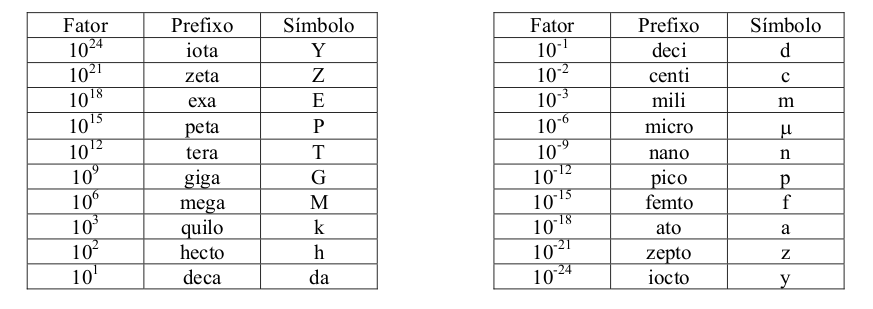
\includegraphics[width=0.85\linewidth]{prefixos.png}

\fbox{\parbox{0.85\linewidth}{\centering
\textbf{[Tabela: prefixos do SI (k, m, $\mu$, n, ...)]}\\
}}
\end{center}
\end{frame}

\begin{frame}{Conversão de unidades mantendo algarismos significativos}
\begin{itemize}
  \item Ex.: se uma medida tem 3 algarismos significativos, a conversão deve manter esses 3.
  \item Evite “colocar zeros à direita” como se isso aumentasse precisão.
\end{itemize}

\begin{block}{Exemplo (ideia)}
Se a medida é \(18{,}7\,\text{dm}\) (3 alg. signif.), então em mm não se deve escrever \(1870\,\text{mm}\),
mas sim algo como \(187\times 10\,\text{mm}\) ou em notação científica \( 1{,}87 \times 10^{3}\,\text{mm}\)(mantendo 3 alg. signif.).
\end{block}
\end{frame}

\begin{frame}{Notação científica}
\begin{itemize}
  \item Forma padrão: um único algarismo (1 a 9) antes da vírgula.
\end{itemize}

\begin{equation}
\label{eq:notacao_cientifica}
x = a \times 10^{n}, \quad 1\le a < 10.
\end{equation}

\begin{block}{Vantagem}
Em notação científica, tendem a aparecer apenas os algarismos significativos (zeros “de posicionamento” somem).
\end{block}
\end{frame}

% =========================================================
\section{Operações com algarismos significativos}

\begin{frame}{Propagação de Erros - Regras gerais}
\begin{itemize}
  \item Em qualquer operação, o resultado \textbf{não pode} ter precisão maior do que a medida “mais pobre”.
  \item Faça a operação normalmente e \textbf{arredonde no final} de acordo com as regras.
\end{itemize}
\end{frame}

\begin{frame}{Adição e subtração}
\begin{block}{Regra (adição/subtração)}
A parte decimal do resultado \textbf{não pode} ter mais casas decimais do que a parcela com \textbf{menos} casas decimais.
\end{block}

\begin{itemize}
  \item Se uma medida está “só até centésimos”, o resultado final também deve estar “só até centésimos”.
\end{itemize}
\end{frame}

\begin{frame}{Multiplicação e divisão}
\begin{block}{Regra (produto/quociente)}
O resultado \textbf{não pode} ter mais algarismos significativos do que o fator (ou termo) \textbf{mais pobre}.
\end{block}

\begin{itemize}
  \item Ex.: \(127{,}8\) (4 alg.) \(\times\) \(11{,}7\) (3 alg.) \(\Rightarrow\) resultado com \textbf{3 alg.} significativos.
\end{itemize}
\end{frame}

\begin{frame}{Critérios de arredondamento (resumo)}
Ao arredondar no primeiro algarismo duvidoso:
\begin{itemize}
  \item Se a parte desprezada \(>\) 5, 50, 500, ... \(\Rightarrow\) aumenta 1 unidade.
  \item Se a parte desprezada \(<\) 5, 50, 500, ... \(\Rightarrow\) mantém.
  \item Se a parte desprezada \(=\) 5, 50, 500, ...:
  \begin{itemize}
    \item algarismo anterior \textbf{ímpar} \(\Rightarrow\) aumenta;
    \item algarismo anterior \textbf{par} (zero incluso) \(\Rightarrow\) mantém.
  \end{itemize}
\end{itemize}
\end{frame}

% =========================================================
\section{Erros experimentais (introdução)}

\begin{frame}{Por que falar de erros?}
\begin{itemize}
  \item Dados experimentais \textbf{sempre} contêm erros.
  \item Uma medida sem incerteza tem pouco significado científico.
  \item Na prática, estimamos um \textbf{erro máximo} (ou desvio) associado.
\end{itemize}
\end{frame}

\begin{frame}{Classificação (visão prática)}
\begin{itemize}
  \item \textbf{Erro de escala}: limitado pela resolução do instrumento.
  \item \textbf{Erro sistemático}: desloca todas as medidas no mesmo sentido; em princípio, pode ser corrigido.
  \item \textbf{Erro aleatório}: flutuações imprevisíveis; tratamos estatisticamente.
\end{itemize}

\begin{equation}
\label{eq:erro_maximo}
\Delta x = \Delta x_{\text{escala}} + \Delta x_{\text{sist}} + \Delta x_{\text{rand}}.
\end{equation}
\end{frame}

% =========================================================
\section{Tratamento estatístico de séries de medidas}

\begin{frame}{Média (valor mais provável)}
Para \(n\) medidas \(x_1,x_2,\ldots,x_n\):
\begin{equation}
\label{eq:media}
\bar{x} = \frac{1}{n}\sum_{i=1}^{n} x_i.
\end{equation}

\begin{itemize}
  \item Em geral, \(\bar{x}\) é uma \textbf{estimativa} do valor verdadeiro.
  \item A qualidade melhora com \(n\) (mais medidas).
\end{itemize}
\end{frame}

\begin{frame}{Desvio de uma medida e desvio médio}
\begin{equation}
\label{eq:desvio_i}
\Delta x_i = x_i - \bar{x},
\end{equation}
e o desvio absoluto:
\begin{equation}
\label{eq:desvio_abs_i}
\abs{\Delta x_i} = \abs{x_i - \bar{x}}.
\end{equation}

\begin{equation}
\label{eq:desvio_medio}
\Delta \bar{x} = \frac{1}{n}\sum_{i=1}^{n}\abs{x_i - \bar{x}}.
\end{equation}

\begin{block}{Comunicação típica}
\[
x = \bar{x} \pm \Delta \bar{x}.
\]
\end{block}
\end{frame}

\begin{frame}{Desvio padrão}
Uma medida de dispersão em torno da média:
\begin{equation}
\label{eq:desvio_padrao}
\sigma = \sqrt{\frac{1}{n-1}\sum_{i=1}^{n}(x_i-\bar{x})^2}.
\end{equation}

\begin{itemize}
  \item \(\sigma\) informa a \textbf{dispersão} das medidas (precisão do conjunto).
  \item Complementa a informação de \(\bar{x}\) (valor mais provável).
\end{itemize}
\end{frame}

% =========================================================
\section{Exercícios}

\begin{frame}{Exercícios I: leituras em instrumentos}
\begin{center}
% >>>>> INSIRA A IMAGEM AQUI (Página com os mostradores/termômetros/réguas) <<<<<
% Sugestão de arquivo: exercicios_I_figuras.png
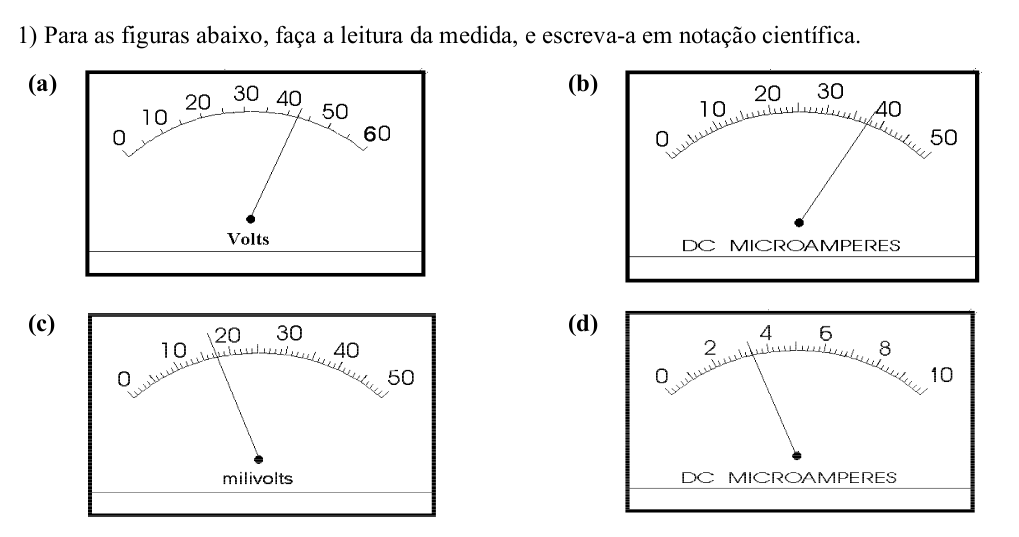
\includegraphics[width=0.92\linewidth]{intrumentos1.png}

\fbox{\parbox{0.92\linewidth}{\centering
\textbf{[Exercícios I: figuras (a)--(i) para leitura e notação científica]}\\
\textit{(Substitua este quadro pela imagem.)}}}
\end{center}
\end{frame}


\begin{frame}
   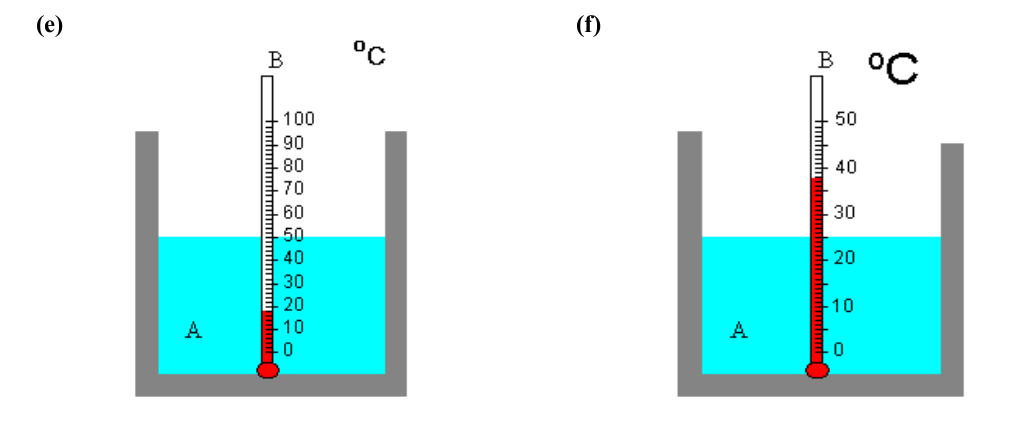
\includegraphics[width=0.92\linewidth]{instrumentos2.png} 
\end{frame}

\begin{frame}{Exercícios I: perguntas conceituais (seleção)}
\begin{enumerate}
  \item O que são algarismos significativos?
  \item O algarismo duvidoso é significativo?
  \item Diferença entre medida direta e indireta.
  \item Zeros à direita e à esquerda: quando contam?
  \item O que significa um instrumento ser mais preciso?
\end{enumerate}
\end{frame}

\begin{frame}{Exercícios II: operações e arredondamento}
\begin{itemize}
  \item Aplique as regras de:
  \begin{itemize}
    \item adição/subtração (casas decimais);
    \item multiplicação/divisão (número de algarismos significativos);
    \item critérios de arredondamento.
  \end{itemize}
  \item Apresente resultados em \textbf{notação científica} e com \textbf{unidades}.
\end{itemize}
\end{frame}


%------------------------------------------------
\section{Exemplo de Adição}
%------------------------------------------------

\begin{frame}{Exemplo 4: Adição de medidas}

Foram medidos os comprimentos de algumas tábuas:

\begin{itemize}
\item 2355,\underline{1} mm
\item 11,\underline{1} dm
\item 117,\underline{3} cm
\item 13,\underline{5} mm
\item 3,\underline{4} dm
\item 77,\underline{5} cm
\item 813,\underline{3} mm
\end{itemize}

Transformando todas as medidas para metros:

\end{frame}

%------------------------------------------------

\begin{frame}{Conversão para metros}

\begin{align*}
2355,\underline{1}\ \text{mm} &= 2,355\underline{1}\ \text{m} \\
11,\underline{1}\ \text{dm} &= 1,1\underline{1}\ \text{m} \\
117,\underline{3}\ \text{cm} &= 1,17\underline{3}\ \text{m} \\
13,\underline{5}\ \text{mm} &= 0,013\underline{5}\ \text{m} \\
3,\underline{4}\ \text{dm} &= 0,3\underline{4}\ \text{m} \\
77,\underline{5}\ \text{cm} &= 0,77\underline{5}\ \text{m} \\
813,\underline{3}\ \text{mm} &= 0,813\underline{3}\ \text{m}
\end{align*}

\end{frame}

%------------------------------------------------

\begin{frame}{Somando as medidas}

\begin{align*}
2,355\underline{1}\ \text{m} \\
+\,1,1\underline{1}\ \text{m} \\
+\,1,17\underline{3}\ \text{m} \\
+\,0,013\underline{5}\ \text{m} \\
+\,0,3\underline{4}\ \text{m} \\
+\,0,77\underline{5}\ \text{m} \\
+\,0,813\underline{3}\ \text{m}
\end{align*}

\[
= 6,57\underline{9}9\ \text{m}
\]

\end{frame}

%------------------------------------------------

\begin{frame}{Aplicando a regra da adição}

A parcela com parte decimal mais pobre é:

\[
0,3\underline{4}\ \text{m}
\]

Logo, o resultado deve ter apenas duas casas decimais.

\[
6,57\underline{9}9\ \text{m}
\]

Arredondando:

\[
6,5\underline{8}\ \text{m}
\]

\end{frame}

%------------------------------------------------
\section{Critérios de Arredondamento}
%------------------------------------------------

\begin{frame}{1º Caso}

Se os algarismos desprezados forem maiores que 5:

\begin{align*}
1524,\underline{5}500100\ \text{cm}^3 &\rightarrow 1524,\underline{6}\ \text{cm}^3 \\
12,1\underline{2}599875\ \text{g} &\rightarrow 12,1\underline{3}\ \text{g} \\
204,\underline{9}6501212\ \text{N} &\rightarrow 205,\underline{0}\ \text{N} \\
0,0012\underline{1}521111\ \text{A} &\rightarrow 0,0012\underline{2}\ \text{A} \\
0,1\underline{3}7298760\ \text{V} &\rightarrow 0,1\underline{4}\ \text{V} \rightarrow 1,\underline{4}\times 10^{-1}\ \text{V}
\end{align*}

\end{frame}

%------------------------------------------------

\begin{frame}{2º Caso}

Se os algarismos desprezados forem menores que 5:

\begin{align*}
69\underline{9},05 &\rightarrow 699 \\
80,\underline{0}32 &\rightarrow 80,0 \\
27,\underline{2}4 &\rightarrow 27,2 \\
4,\underline{8}205 &\rightarrow 4,8 \\
0,5\underline{4}31 &\rightarrow 0,54
\end{align*}

\end{frame}

%------------------------------------------------

\begin{frame}{3º Caso}

Se o número desprezado for exatamente 5:

\begin{itemize}
\item Se o algarismo anterior for \textbf{ímpar}, aumenta.
\item Se for \textbf{par}, permanece.
\end{itemize}

Exemplos:



\[
\begin{array}{lcl}
1,5\underline{5}500\ \text{Wb/m}^2 & \ldots\ldots\ldots\ldots\ldots & 1,56\ \text{Wb/m}^2 \\

0,003\underline{5}5\ \text{cal/g} & \ldots\ldots\ldots\ldots\ldots & 
0,0036\ \text{cal/g} = 3,6\times10^{-3}\ \text{cal/g} \\

129,\underline{5}00\ \text{g/s} & \ldots\ldots\ldots\ldots\ldots & 
130\ \text{g/s} = 1,30\times10^{2}\ \text{g/s} \\

1,9\underline{5}00\ \text{dyn/cm}^2 & \ldots\ldots\ldots\ldots\ldots & 
2,0\ \text{dyn/cm}^2 \\

0,80\underline{5}\ \text{N/m} & \ldots\ldots\ldots\ldots\ldots & 
0,80\ \text{N/m} = 8,0\times10^{-1}\ \text{N/m} \\

25,10\underline{5}\ \text{mm-Hg} & \ldots\ldots\ldots\ldots\ldots & 
25,10\ \text{mm-Hg} = 2,510\times10^{-1}\ \text{mm-Hg} \\

2\underline{6}500\ \text{m} & \ldots\ldots\ldots\ldots\ldots & 
2,6\times10^{4}\ \text{m} \\

2\underline{8},500\ \text{J} & \ldots\ldots\ldots\ldots\ldots & 
28\ \text{J} = 2,8\times10^{1}\ \text{J} \\

0,000\underline{4}500\ \text{N.m} & \ldots\ldots\ldots\ldots\ldots & 
0,0004\ \text{N.m} = 4\times10^{-4}\ \text{N.m} \\

9,\underline{5}0000\ \text{C/g} & \ldots\ldots\ldots\ldots\ldots & 
1\times10^{1}\ \text{C/g}
\end{array}
\]



\end{frame}
% =========================================================
\section{Fechamento}

\begin{frame}{Resumo}
\begin{itemize}
  \item Medidas sempre exigem \textbf{unidade} e \textbf{incerteza}.
  \item Algarismos significativos = dígitos certos + 1 duvidoso.
  \item Conversão de unidades \textbf{não pode} alterar precisão.
  \item Operações: resultado limitado pela medida “mais pobre”.
  \item Em séries de medidas: \(\bar{x}\), desvios e \(\sigma\) organizam a comunicação científica.
\end{itemize}
\end{frame}

%------------------------------------------------
\section{Subtração}
%------------------------------------------------

\begin{frame}{Regra para a subtração}

Do ponto de vista das operações matemáticas, a subtração é idêntica à
adição de números relativos.

\begin{block}{Regra}
O resultado da subtração de várias medidas de uma mesma grandeza física
não pode ter maior número de algarismos significativos, na sua parte
decimal, do que a parte decimal mais pobre das parcelas.
\end{block}

\end{frame}

%------------------------------------------------

\begin{frame}{Exemplo 5}

Uma tábua tem comprimento:

\[
2859,0 \ \text{mm}
\]

São cortados pedaços de:

\[
12,3\ \text{dm},\qquad
113,7\ \text{cm},\qquad
63,5\ \text{mm}
\]

Transformando para metros:

\[
2,859\underline{0}\ \text{m},\quad
1,2\underline{3}\ \text{m},\quad
1,13\underline{7}\ \text{m},\quad
0,063\underline{5}\ \text{m}
\]

\end{frame}

%------------------------------------------------

\begin{frame}{Subtração}

\[
\begin{array}{r}
2,859\underline{0}\ \text{m} \\
-\,1,2\underline{3}\ \text{m} \\
-\,1,13\underline{7}\ \text{m} \\
-\,0,063\underline{5}\ \text{m} \\
\hline
0,4\underline{285}\ \text{m}
\end{array}
\]

Aplicando a regra dos algarismos significativos:

\[
0,4\underline{2}|85 \ \text{m}
\]

\[
0,43\ \text{m}
\]

\end{frame}

%------------------------------------------------

\begin{frame}{Interpretação}

O primeiro algarismo duvidoso à esquerda é o

\[
\underline{2}
\]

Logo:

\[
0,42|85 \approx 0,43
\]

O resultado final tem o algarismo duvidoso na casa dos centímetros.

\end{frame}

%------------------------------------------------

\begin{frame}{Contra-exemplo}

Considere:

\[
1592,0\ \text{mm}
\]

São cortados pedaços de:

\[
12,3\ \text{dm},\qquad
36,1\ \text{cm}
\]

Transformando:

\[
1,592\underline{0}\ \text{m},\quad
1,2\underline{3}\ \text{m},\quad
0,36\underline{1}\ \text{m}
\]

\end{frame}

%------------------------------------------------

\begin{frame}{Subtração}

\[
\begin{array}{r}
1,592\underline{0}\ \text{m} \\
-\,1,2\underline{3}\ \text{m} \\
-\,0,36\underline{1}\ \text{m} \\
\hline
0,0\underline{010}\ \text{m}
\end{array}
\]

Aplicando a regra:

\[
0,0\underline{0}|10
\]

\[
0,00\ \text{m}
\]

\end{frame}

%------------------------------------------------

\begin{frame}{Observação}

Neste caso as conclusões sobre a precisão ficam prejudicadas.

Isso ocorre quando os valores subtraídos são muito próximos.

\end{frame}

%------------------------------------------------

\begin{frame}{Exemplos de aplicação}

\begin{align*}
138,94\,m - 12,3\,m &= 126,64\,m = 126,6\,m = 1,266\times10^{2}\,m \\
118,57\,s - 58,303\,s &= 60,267\,s = 60,27\,s = 6,027\times10^{1}\,s \\
5,00\,g - 2,016\,g &= 2,984\,g = 2,98\,g \\
0,00015\,A + 0,072\,A - 0,091\,A - 0,0593\,A &= -0,07815\,A = -0,078\,A \\
1,0000\,m^2 - 0,633\,m^2 + 0,5\,m^2 - 0,27\,m^2 &= 0,597\,m^2 = 0,6\,m^2
\end{align*}

\end{frame}

%------------------------------------------------

\begin{frame}{Regra geral}

\begin{block}{Importante}
Tanto na adição quanto na subtração, o arredondamento é executado
\textbf{após a operação}, de acordo com a medida menos precisa.
\end{block}

\end{frame} 



%------------------------------------------------
\section{Multiplicação}
%------------------------------------------------

\begin{frame}{Multiplicação - Exemplo 7}

Medindo os lados de um retângulo com réguas diferentes:

\begin{center}
\begin{tabular}{ccc}
Régua & Lado a & Lado b\\
\hline
decimetrada & 12,8 dm & 1,2 dm\\
centimetrada & 127,\underline{8} cm & 11,\underline{7} cm\\
milimetrada & 1279,\underline{1} mm & 117,\underline{4} mm
\end{tabular}
\end{center}

Queremos calcular a área do retângulo.

\end{frame}

%------------------------------------------------

\begin{frame}{Cálculo da área}

\begin{center}
\begin{tabular}{cc}
Régua & Área = a.b \\
\hline
decimetrada & $12,8 \times 1,2 = 15,36\ dm^2 = 15\ dm^2$ \\
centimetrada & $127,8 \times 11,7 = 1495,26\ cm^2 = 150 \times 10^1\ cm^2$ \\
milimetrada & $1279,1 \times 117,4 = 150166,34\ mm^2 = 1502 \times 10^2\ mm^2$
\end{tabular}
\end{center}

\end{frame}



\begin{frame}{Regra para multiplicação}

\begin{block}{Regra}

O resultado da multiplicação de várias medidas não pode ter maior número
de algarismos significativos do que o fator **mais pobre**.

\end{block}

Exemplo anterior:

\[
127,\underline{8} \rightarrow 4\ alg.\ significativos
\]

\[
11,\underline{7} \rightarrow 3\ alg.\ significativos
\]

Logo o resultado terá **3 algarismos significativos**.

\end{frame}

%------------------------------------------------

\begin{frame}{Exemplos}

\begin{align*}
1,52834\,dm \times 3,38\,cm &= 0,51657892\,dm^2 \\
&= 0,517\,dm^2 \\
&= 5,17\times10^{-1}\,dm^2
\end{align*}

\begin{align*}
832\,N/m \times 0,25\,m^2 &= 208\,N.m \\
&= 2,1\times10^2\,J
\end{align*}

\begin{align*}
0,315\,\mu A \times 5327\,m\Omega
&= 1,678005\times10^{-6}V \\
&= 1,68\,\mu V
\end{align*}

\end{frame}

%------------------------------------------------

\begin{frame}{Mais exemplos}

\begin{align*}
(8,3\,K)^4 &= 4745,8321\,K^4 \\
&= 4,7\times10^3\,K^4
\end{align*}

\begin{align*}
0,0001\,m \times 0,0198\,m \times 0,77\,m
&= 1,5246\times10^{-6}\,m^3 \\
&\approx 2\times10^{-6}\,m^3
\end{align*}

\end{frame}


\end{document}